% ============================================================
% IE UNIVERSITY - BAM - ML & Communication Skills FINAL REPORT
% FIRST DRAFT v2 (structure + numbers). Prose is a placeholder that the
% authors will rewrite themselves (course policy: AI may not write the
% submitted prose). Red [TODO] marks things to decide/verify.
%
% Changes driven by the Sentence Outline feedback (40/40):
%  - Methods and results in parallel, per model family (Sec. 4)
%  - citations numbered by order of first appearance (unsrtnat), first = [1]
%  - more related work (Sec. 2)
%  - pending analyses completed or their effect on conclusions stated (Sec. 6)
%  - computing setup in the Methodology (Sec. 4.1)
%  - figures regenerated at column width (scripts/make_report_figures.py)
% ============================================================

\documentclass[clean,twocolumn]{bam-proposal}

\newcommand{\todo}[1]{{\color{red}[TODO: #1]}}

\BAMdeliverable{Final Report}
\BAMtitle{Early Collision Risk Forecasting from ESA Conjunction Data Messages}
\BAMteam{Pedro Jon Fuentes Garc\'es; Mario Fern\'andez Velasco}
\BAMcourse{Machine Learning \& Communication Skills}
\BAMacademicyear{2026--2027}
\BAMsubmissiondate{25 November 2026}

% numbered in order of first citation, so the first cited source is [1]
\BAMbibliographystyle{unsrtnat} % \todo{switch to an MLA .bst if the course template requires it}
\BAMbibliographyfile{references}

\newcommand{\HR}{\mathrm{HR}}
\newcommand{\LRP}{\textsc{lrp}}
\newcommand{\CRP}{\textsc{crp}}
\newcommand{\MSEHR}{\mathrm{MSE}_{\mathrm{HR}}}

\begin{document}
\twocolumn[\makeproposalheader]

% ------------------------------------------------------------
\begin{abstract}\noindent
\small
Operators receive Conjunction Data Messages (CDMs) warning of close approaches between orbiting objects, and a few of them reach a risk high enough to justify a manoeuvre. Using the ESA Collision Avoidance Challenge data, we ask whether any learned model that sees only CDMs received at least two days before the time of closest approach (TCA) improves on simply repeating the latest reported risk (LRP), and whether a calibrated two-stage design characterises risk jumps better. We build an event-level evaluation protocol (repeated stratified 5-fold CV, BCa bootstrap, one-shot official test) and compare OLS, ridge, lasso, $k$-NN, kernel ridge, random forest, gradient boosting, an MLP, a GRU and nine two-stage combinations. Under the challenge metric no learned model beats LRP, neither internally nor on the official test (LRP: $L=0.694$; best learned, gradient boosting: $L=1.458$). Under an unclipped version of the same metric the tree ensembles are roughly an order of magnitude better than LRP, which shows how much the conclusion depends on how a missed high-risk event is penalised. A failure atlas and a lead-time analysis explain where and why models fail. \todo{rewrite abstract once the story is final}
\end{abstract}

% ------------------------------------------------------------
\section{Introduction}

\todo{Context paragraph: debris, conjunction assessment, why early warning matters.}
Operators of satellites receive Conjunction Data Messages (CDMs) that describe a predicted close approach between two objects and an estimated collision risk. The risk estimate is refreshed several times a day until the TCA; whether to manoeuvre must be decided a couple of days before, when the information is still uncertain. The ESA Kelvins Collision Avoidance Challenge \citep{kelvins2019challenge,uriot2021collision} turned this into a forecasting task: given the CDMs of an event received at least two days before TCA, predict the (log$_{10}$) risk in the last CDM. The winning solutions barely beat the trivial \emph{latest risk prediction} (LRP), which just repeats the risk of the last available CDM \citep{uriot2021collision}.

We pose two research questions.
\textbf{RQ1:} using only CDMs with time to TCA $\ge 2$ days, which modelling approach, if any, improves on LRP under the challenge metrics $F_2$, $\MSEHR$ and $L=\MSEHR/F_2$?
\textbf{RQ2:} does a calibrated two-stage model (calibrated probability of high risk, then a magnitude regressor) characterise events whose risk jumps close to TCA better than single-stage models?
Because LRP is so hard to beat, we treat the \emph{protocol} (what is predicted, from which messages, on which events, judged how) as a contribution in itself, and we measure success by the quality of the evidence rather than by beating the leaderboard.

\paragraph{Contributions.}
(i) An event-level protocol that removes a label/input overlap present in a quarter of the training events (Sec.~\ref{sec:data}). (ii) A like-for-like comparison of ten model families against LRP, with paired bootstrap intervals and a one-shot official test (Secs.~\ref{sec:methods} and~\ref{sec:official}). (iii) A derivation of a training-target floor that lets squared-error trees and networks raise an alarm at all (Sec.~\ref{sec:trees}). (iv) A failure atlas, a lead-time curve and a leave-one-mission-out check (Secs.~\ref{sec:atlas} and~\ref{sec:lead}).

% ------------------------------------------------------------
\section{Background and Related Work}\label{sec:background}

\paragraph{The challenge and its metric.}
The Kelvins challenge ranks predictions by $L=\MSEHR/F_2$, where $F_2$ weights recall over precision for the high-risk (HR) class and $\MSEHR$ is the squared error of the predicted log-risk over truly HR events, with predictions clipped at $-6.001$ \citep{uriot2021collision}. A missed HR event is therefore costlier than a false alarm, and with few HR events a handful of cases can reorder two models. The organisers report that the simple latest-risk baseline was very hard to beat \citep{uriot2021collision}. \todo{one sentence on how the top teams did and what they used.}

\paragraph{Machine learning for conjunction assessment.}
Besides the competition report, learned models have been applied to the same CDM data, for example Bayesian deep learning that outputs uncertainty about the predicted risk \citep{pinto2020towards}. \todo{read and summarise 2--3 more papers (e.g.\ competition winners) and say what we do differently: a fixed protocol that removes label/input overlap, a one-shot official test, and an explicit comparison of the metric clipping.}

\paragraph{Rare-event evaluation, thresholds and calibration.}
With about 1\% positives, accuracy is uninformative and precision--recall-based summaries are preferred over ROC curves \citep{saito2015precision}. For $F_1$, the optimal decision threshold on a calibrated probability is half the optimal score \citep{lipton2014optimal}; we use the analogous threshold $F^*/(1+\beta^2)$ for $F_2$ (our extension, checked by simulation, not stated in that paper) to set the training-target floor of the tree and neural models (Sec.~\ref{sec:trees}). Classifier scores can be turned into probabilities with Platt scaling \citep{platt1999probabilistic}, and the quality of a probabilistic forecast is measured with the Brier score \citep{brier1950verification} and reliability diagrams; calibration is known to depend on the learner \citep{niculescu2005predicting}. \todo{state the $F_\beta$ generalisation as ours and show the one-line derivation or the simulation.}

\paragraph{Trees versus networks on tabular data.}
On medium-sized tabular data, tree ensembles are often at least as good as neural networks \citep{grinsztajn2022tree,shwartz2022tabular}. This motivates treating the networks of Sec.~\ref{sec:nn} as a fair ablation rather than as our main model, and it frames the comparison of Table~\ref{tab:oof}.

\paragraph{Uncertainty.}
We report 95\% BCa bootstrap intervals \citep{efron1987bca} over events and paired differences with LRP, since with 93 HR events a point estimate alone would overstate what the data resolve.

% ------------------------------------------------------------
\section{Data and Evaluation Protocol}\label{sec:data}

\paragraph{Data.}
We use the public Kelvins data \citep{zenodo4463683} (CC BY 4.0): 13{,}154 training events, each a time series of CDMs with the risk estimate, miss distance, relative speed, orbit-determination quality and object type of the second object. The official test set has 2{,}167 events, 150 of them HR (6.9\%); its final risk values are private labels. An event is \emph{high risk} (HR) if its final risk is at least $10^{-6}$, i.e.\ $-6$ in log$_{10}$.

\paragraph{Unit, label, inputs.}
The unit is the event. The label is the log-risk of the last CDM (\texttt{risk\_final}), with $y_{\HR}=\mathbb 1\{\texttt{risk\_final}\ge -6\}$ derived from it. Inputs are restricted to CDMs with time to TCA $\ge2$ days (Fig.~\ref{fig:timeline}). About 80\% of events sit at the $-30$ floor of the risk scale.

\paragraph{Event filter.}\label{sec:filter}
In 3{,}032 training events the last CDM itself lies $\ge2$ days before TCA, so the label is also an input and LRP reproduces it exactly ($F_2=1$, $L=0$). These events hold 228 of the 321 HR events (71\%). We exclude them, together with 1{,}212 events with no usable CDM, and keep \textbf{8{,}892 events with 93 HR (1.05\%)}. 599 of them (27 HR) have their last CDM one to two days before TCA; they are easier for LRP, so the internal validation is somewhat optimistic. For the official test we keep every event with at least one CDM at $\ge2$ days. HR prevalence is 1.05\% internally against 6.9\% in the test, so internal and official numbers are never directly comparable.

\paragraph{Features and jump taxonomy.}
Each event becomes one row of 35 features computed from usable CDMs only: risk at the first and last messages and at three intermediate quantiles; risk minimum, maximum, range, mean and standard deviation; the same snapshots for miss distance, relative speed and orbit-determination quality; message counts and timing; and a one-hot object type. The mission identifier is excluded to avoid mission-specific shortcuts. For analysis only, each event is labelled \emph{stable-low}, \emph{stable-high}, \emph{jump-up} or \emph{jump-down} from $\Delta=\texttt{risk\_final}-\LRP$ with a symmetric cut of one order of magnitude (Fig.~\ref{fig:imbalance}); the taxonomy is never an input, target or weight.

\begin{figure}[t]
  \centering
  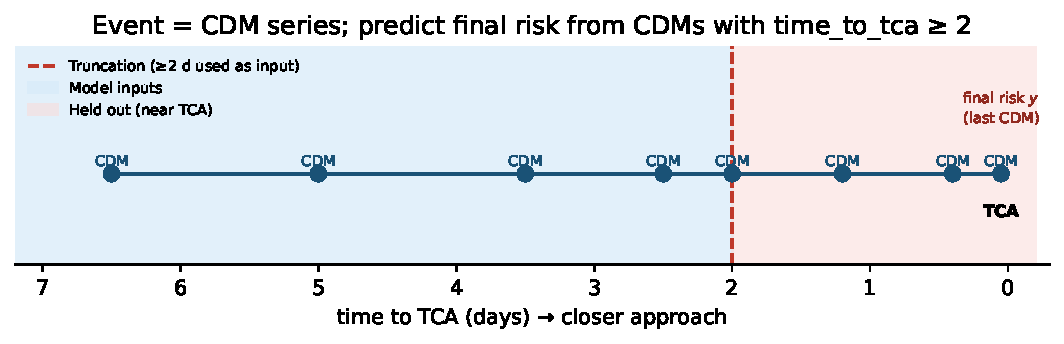
\includegraphics[width=0.92\columnwidth]{figures/fig_cdm_timeline.pdf}
  \caption{Schematic event. Inputs use only CDMs with time to TCA $\ge2$ days; the label is the risk of the last CDM, which in the retained events arrives within two days of TCA.}
  \label{fig:timeline}
\end{figure}

\begin{figure*}[t]
  \centering
  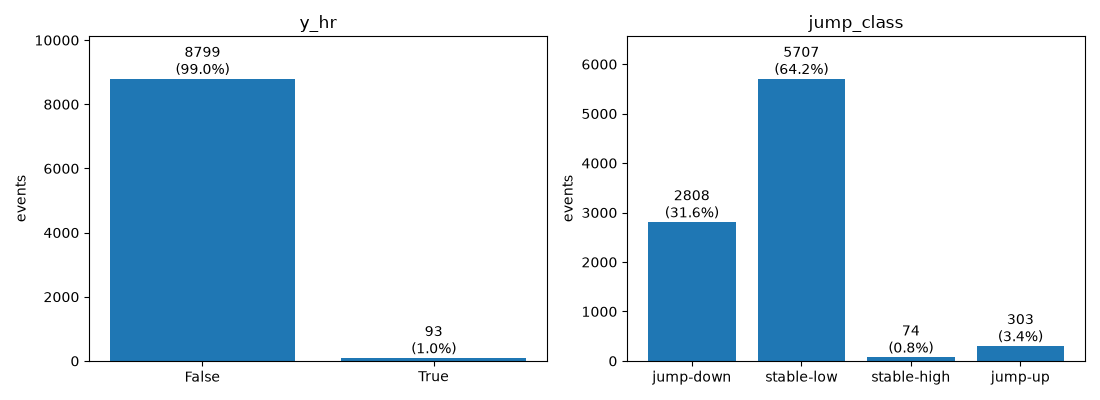
\includegraphics[width=0.75\textwidth]{figures/fig_imbalance.png}
  \caption{Retained event set (8{,}892 events). Left: HR class imbalance (HR = final risk $\ge-6$). Right: jump taxonomy with a cut of one order of magnitude between the last usable risk and the final risk; analysis only. \todo{check fonts are legible; regenerate with larger labels if not}}
  \label{fig:imbalance}
\end{figure*}

% ------------------------------------------------------------
\section{Methodology and Results by Model Family}\label{sec:methods}

Each subsection pairs the method with its result, in the same order as the rows of Table~\ref{tab:oof}, so that families can be compared directly. Every modelling choice is recorded as a decision record in the repository (\texttt{docs/decisions/}) with the deciding member's justification; code only uses registered parameters.

\subsection{Shared protocol and computing setup}\label{sec:protocol}
\textbf{Cross-validation.} All internal comparisons use event-level 5-fold CV stratified on $y_{\HR}$ (18--19 HR events per validation fold), repeated $R=5$ times (seeds 42--46); out-of-fold (OOF) predictions are scored and metrics averaged over repetitions. Kernel ridge uses $R=2$ for cost. Preprocessing and hyper-parameters are fitted inside the training part only; selection uses an inner CV.

\textbf{Metrics.} $F_2$ with the alarm $\hat r\ge-6$; $\MSEHR$; $L=\MSEHR/F_2$ (lower is better). We report the challenge's \emph{clipped} $\MSEHR$ and $L$, and an \emph{unclipped} version, because the choice changes the ranking (Sec.~\ref{sec:compare}). Intervals: event bootstrap ($B=10{,}000$, seed 2026), 95\% BCa, paired differences against LRP.

\textbf{Official test.} Used once, at the end, with models frozen: for each learned model the hyper-parameter selection is re-run on the full filtered training set (inner seed 42) and a single model is fitted on it; no fold ensemble, and the test never enters selection. Official and internal results appear in separate tables (Tables~\ref{tab:official} and~\ref{tab:oof}).

\textbf{Computing setup.} All experiments ran on CPU on a single laptop-class machine (AMD Ryzen 5 PRO 215, 12 logical cores, 7 GB RAM available under WSL2, no GPU) with Python 3.12, scikit-learn 1.9 \citep{pedregosa2011sklearn}, PyTorch 2.15 (CPU) \citep{paszke2019pytorch}, NumPy 2.2, pandas 3.0 and SciPy 1.17. Wall times of the internal runs (25 outer fits each) were under a minute for lasso and $k$-NN, about 30 min for the MLP, 1\,h for kernel ridge (two repetitions), 1.7\,h for the GRU, and 11.6\,h for the $L_1$ stage-1 classifier; on the full training set, the single official fits took 1 min (RF), 5 min (GBDT) and 23 min (GRU). Seeds, package versions (\texttt{requirements.txt}) and the scripts that regenerate every table are in the repository. \todo{confirm both authors ran with these versions; confirm the GBDT/RF OOF times.}

\subsection{Baselines: CRP and LRP}
CRP (constant risk prediction) predicts one value for all events; LRP repeats the risk of the last usable CDM. LRP is the baseline against which every comparison is paired. Internally $F_2=0.492$, clipped $L=0.548$ and unclipped $L=24.7$; the unclipped value is large because LRP predicts the $-30$ floor for events that later reach HR.

\subsection{Linear models, $k$-NN and kernel ridge}
\textbf{Method.} OLS, ridge \citep{hoerl1970ridge} and lasso \citep{tibshirani1996lasso} regress \texttt{risk\_final} on standardised features; the penalty is chosen by nested 5-fold CV using average precision of $\hat r$ against $y_{\HR}$. $k$-NN and kernel ridge (RBF kernel, $\gamma=10/m$ with $m$ the median squared distance of the training part, ridge penalty by inner CV) use the same target and preprocessing. Their continuous predictions almost never reach $-6$, so each uses an alarm threshold chosen on its training fold to maximise $F_2$; this makes their $F_2$ not strictly comparable with LRP's fixed line (flagged in Table~\ref{tab:oof}).

\textbf{Result.} Lasso is the only one that matches LRP on $F_2$ ($0.486$ $[0.413,0.557]$; paired difference $-0.006$, CI $[-0.057,0.034]$), but its error on HR events is large: clipped $L=2.40$ $[1.80,3.45]$, paired $+1.86$ $[1.28,2.86]$ above LRP. OLS, ridge, $k$-NN and kernel ridge are well below LRP ($F_2$ between $0.20$ and $0.28$). The linear models, $k$-NN and (almost) kernel ridge share the same clipped $\MSEHR$ ($1.161$) because their predictions for every HR event fall below $-6$ and are clipped, so their differences come only from $F_2$.

\subsection{Tree ensembles and the target floor}\label{sec:trees}
\textbf{Method.} Random forests \citep{breiman2001random} and gradient boosting \citep{friedman2001greedy} regress \texttt{risk\_final}. The first runs gave $F_2=0$ (RF) and $F_2\approx0.07$ (GBDT): with 80\% of events at the $-30$ floor, a leaf mean never reaches $-6$ however much capacity we add. If a leaf has HR fraction $p$, its prediction is approximately $p\,\mu_{\HR}+(1-p)\,m(c)$ when the target is floored at $c$, and it alarms iff $p\ge p^*(c)$; choosing $c$ is choosing the HR fraction needed to alarm. We set $p^*=F^*/5$, the $F_2$ analogue of the $F_1$ result of \citet{lipton2014optimal} (their threshold is half the optimal score), with $F^*$ the LRP $F_2$ on the training fold, and solve for $c\approx-6.09$ per fold. Models are fitted on $\max(\texttt{risk\_final},c)$; evaluation uses the original labels, and revocation criteria R0--R4 are computed from OOF predictions after each run.

A second iteration added sample weights $w$ on HR events with $c(w)$ recomputed so that $-6$ remains the $F_2$-optimal line. $w\in\{1,2,5,10\}$ and, for trees, the number of trees in $\{300,500,1000\}$ are selected per outer fold by nested 3-fold CV on pooled unclipped $L$.

\textbf{Result.} RF and GBDT have the lowest clipped $L$ among learned models ($1.85$ and $1.87$) and remain more than three times above LRP; $F_2$ is $0.436$ and $0.417$. The weights barely mattered: GBDT chose $w=1$ in all 25 outer fits and RF in 21, so iteration 2 moved $F_2$ by less than $0.003$. Both rely mainly on summaries of the risk history (Fig.~\ref{fig:importance}); geometry and object type contribute little, which suggests the models mostly re-learn what LRP already uses. Impurity and permutation importances agree on the family but not on the order, and the leading features are strongly correlated (pairwise $|r|$ up to 0.94), so we claim no ranking; importances are not causal.

\begin{figure}[t]
  \centering
  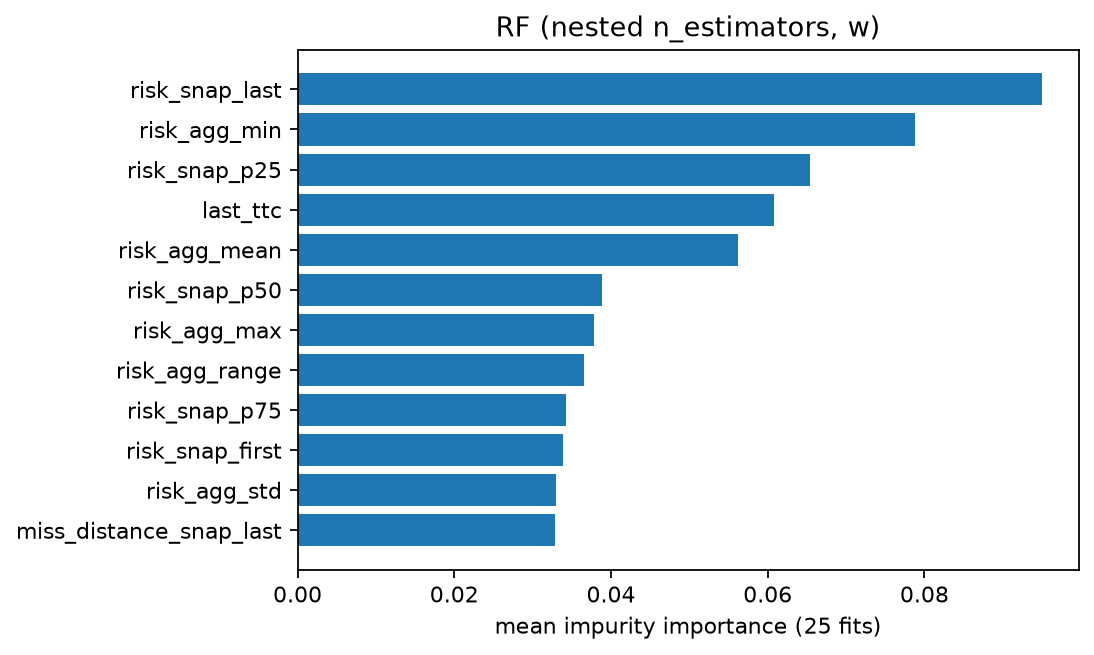
\includegraphics[width=0.95\columnwidth]{figures/fig_importance_rf.png}
  \caption{Random forest impurity importances averaged over 25 fold fits (top features). Not causal. \todo{show GBDT in the same panel or drop}}
  \label{fig:importance}
\end{figure}

\subsection{Neural networks (ablation)}\label{sec:nn}
\textbf{Method.} A tabular MLP ($128\to64\to1$) takes the same 35 features; a GRU \citep{cho2014gru} (hidden 64, last valid state, sequence length $T=20$) takes the masked sequence of usable CDMs. Both regress \texttt{risk\_final} with the floor and the weights above, a weighted mean squared loss, Adam \citep{kingma2015adam} (learning rate $10^{-3}$, batch 64), up to 100 epochs, early stopping with patience 10 on a weighted validation loss, and the same nested selection of $w$ (it chose $w\ge2$ in 24 of 25 outer fits for the MLP and in all 25 for the GRU). They are an ablation, not the main claim.

\textbf{Result.} Iteration 2 improved them a lot (GRU: $F_2$ $0.036\to0.330$, clipped $L$ $49.3\to2.45$; MLP: $0.217\to0.308$, $5.30\to3.29$), but the intervals are wide (GRU $F_2$ $[0.27,0.39]$, $L$ $[1.75,3.66]$; MLP $F_2$ $[0.26,0.37]$, $L$ $[2.34,4.94]$) and neither network reaches the trees, in line with the tabular-data literature \citep{grinsztajn2022tree,shwartz2022tabular}.

\subsection{Calibrated two-stage model}\label{sec:twostage}
\textbf{Method.} Stage 1 is a logistic classifier (unpenalised, L2 or L1; strength by inner-CV AUC with the one-standard-error rule) with balanced class weights, and its log-odds score is calibrated with Platt scaling on the out-of-fold scores of the inner CV. Stage 2 is one of OLS, ridge or lasso, trained on all events (not only HR) so it does not over-predict on low-risk events. All $3\times3$ pairs are evaluated to see what each stage contributes. The alarm is $p\ge t$ with $t$ maximising $F_2$ on the training fold; the predicted risk is the stage-2 output. Calibration is measured with the Brier score and ten equal-count bins.

\textbf{Result.} The probabilities are better than a constant: Brier $0.0095$ (unpenalised), $0.0093$ (L2) and $0.0089$ (L1), against $0.0103$ for the HR rate; in the top decile for L1 the mean prediction is $0.090$ and the observed HR frequency $0.092$ (Fig.~\ref{fig:reliability}). As a system, however, the best pair (L1 + lasso) has $F_2=0.420$ $[0.353,0.484]$ and $L=2.77$ $[2.10,3.77]$: above OLS in $F_2$ (paired $+0.156$ $[0.101,0.208]$), below lasso ($-0.066$ $[-0.127,-0.007]$) and below LRP ($-0.072$ $[-0.128,-0.020]$). Because stage 2 is the same regressor, clipped $\MSEHR$ is unchanged; the first stage improves the \emph{alarm}, not the \emph{magnitude}, and stage 2 is the bottleneck. The selected L1 strength lies on the edge of the grid in all fits and the L2 strength often does (a limitation).

\begin{figure}[t]
  \centering
  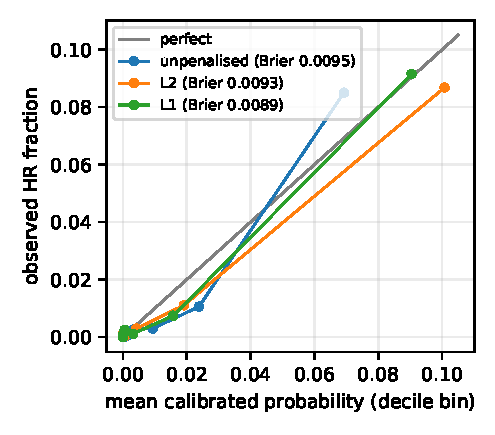
\includegraphics[width=\columnwidth]{figures/fig_reliability.pdf}
  \caption{Reliability of the calibrated stage-1 probabilities: mean predicted probability against observed HR fraction in ten equal-count bins, averaged over the five repetitions. The diagonal is perfect calibration; most events fall in the low-probability bins near the origin.}
  \label{fig:reliability}
\end{figure}

\subsection{Comparison across models}\label{sec:compare}
Table~\ref{tab:oof} collects the internal results. Under the challenge metric \textbf{no learned model beats LRP}. The ranking changes under the unclipped metric: LRP predicts $-30$ for about 80\% of events, which is a huge error for HR events whose last usable risk is at the floor (unclipped $L=24.7$), against $1.93$ (RF) and $1.96$ (GBDT). The trees are about ten times better than LRP when a missed HR event is penalised by its real distance, while the linear models are hundreds of times worse because their unclipped error on HR events is dominated by predictions far below $-6$. We report both and do not claim that one is the right metric: the challenge metric rewards \emph{not being badly wrong in the dangerous region}; the unclipped one rewards \emph{being close}. \todo{decide which is the headline metric.}

\begin{table}[t]
\centering\footnotesize
\caption{Internal protocol: 8{,}892 events, 93 HR; OOF means of $5\times5$-fold CV. Higher $F_2$ and lower $\MSEHR$, $L$ are better; ``clip.'' uses predictions clipped at $-6.001$. Intervals are in the text (RF/GBDT intervals not computed yet). $^{a}$alarm threshold fitted per training fold; the others alarm at $-6$. $^{b}$two repetitions. $^{c}$best of nine pairs by $F_2$: L1 logistic + lasso.}
\label{tab:oof}
\setlength{\tabcolsep}{3pt}
\begin{tabular}{@{}lcccc@{}}
\toprule
Model & $F_2$ & $\MSEHR$ clip. & $L$ clip. & $L$ unclip. \\
\midrule
CRP & 0.050 & 0.475 & 9.46 & 9.46 \\
LRP & 0.492 & \textbf{0.270} & \textbf{0.548} & 24.7 \\
\midrule
OLS$^{a}$ & 0.264 & 1.161 & 4.41 & 741 \\
Ridge$^{a}$ & 0.284 & 1.161 & 4.11 & 1019 \\
Lasso$^{a}$ & 0.486 & 1.161 & 2.40 & 645 \\
$k$-NN$^{a}$ & 0.270 & 1.161 & 4.30 & 928 \\
Kernel ridge$^{a,b}$ & 0.199 & 1.148 & 5.77 & 1012 \\
\midrule
Random forest & 0.436 & 0.808 & 1.85 & \textbf{1.93} \\
Grad.\ boosting & 0.417 & 0.779 & 1.87 & 1.96 \\
MLP & 0.308 & 1.005 & 3.29 & 4.08 \\
GRU & 0.330 & 0.805 & 2.45 & 3.34 \\
\midrule
Two-stage$^{a,c}$ & 0.420 & 1.161 & 2.77 & 742 \\
\bottomrule
\end{tabular}
\end{table}

\subsection{Failure atlas}\label{sec:atlas}
\textbf{Method.} Cases are selected by rules written before any case was inspected, on OOF predictions only (never the official test), requiring the contrast in at least 3 of the 5 repetitions: HR events that LRP misses and a tree model catches (C1) and the reverse (C2); events where most syllabus models contradict LRP (C3, C4); three jump cases with different outcomes (C5--C7); and a multi-model failure (C8). Ties go to the largest true risk. Slots with an empty candidate pool are reported as empty, not relaxed: the slot for a failure that calibration turns into a success (O2) is empty.

\textbf{Result.} Eight core and two optional cases were found. \textbf{C5}: the last usable risk is at the $-30$ floor and the final risk is $-5.75$ (a jump of about $+24$ orders of magnitude); LRP is wrong by construction \todo{check in the timeline whether any input anticipates the jump}. \textbf{C6, C7}: jump-down events in which LRP predicts a dangerous risk that disappears. \textbf{C3}: a jump-up that LRP misses and the syllabus models catch. \textbf{C8}: a multi-model failure with a $+2.1$ jump. \todo{one paragraph per two or three cases with Fig.~\ref{fig:atlas}; only claim that hard cases are mostly unanticipated jumps if the atlas supports it; with eight selected cases it illustrates, not counts.} Because the O2 pool is empty, we have no evidence that calibration helps on jumps (Sec.~\ref{sec:status}).

\begin{figure}[t]
  \centering
  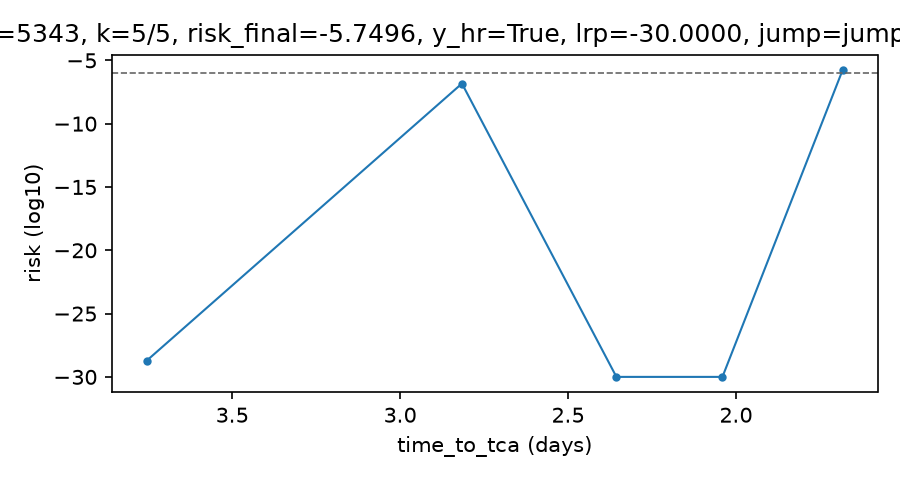
\includegraphics[width=\columnwidth]{figures/fig_atlas_c5.png}
  \caption{Atlas case C5: CDM risk timeline of a jump-up event (last usable risk at the floor, final risk $-5.75$) with the predictions of each model. \todo{pick 1--2 panels, redraw at column width with larger fonts if needed}}
  \label{fig:atlas}
\end{figure}

\subsection{Lead time and leave-one-mission-out}\label{sec:lead}
\textbf{Method.} We repeat the protocol with inputs restricted to CDMs at least $t_{\mathrm{cut}}\in\{2,3,4\}$ days before TCA for LRP, GBDT and the best linear model, re-selecting hyper-parameters at each cut (events without a CDM that early are dropped, so HR events fall from 93 to 74 and 68). The leave-one-mission-out check uses the same three rows with 19 folds by mission; folds whose held-out mission has no HR event are skipped and recorded.

\textbf{Result.} The error grows as the earliest usable CDM moves back (Fig.~\ref{fig:leadtime}): unclipped $L$ of GBDT goes $1.96\to3.08\to3.89$ and that of LRP $24.7\to51.6\to69.6$. Six of the 19 missions have no HR event; over the remaining 13 the mean unclipped $L$ is $1.34$ for GBDT and $4.67$ for LRP (means over the folds where it is finite), so the advantage of trees under the unclipped metric is not specific to one mission. \todo{add per-mission spread; say which folds had infinite $L$.}

\begin{figure}[t]
  \centering
  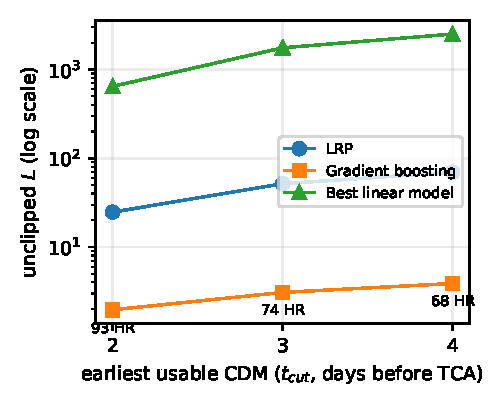
\includegraphics[width=\columnwidth]{figures/fig_leadtime.pdf}
  \caption{Lead-time analysis: unclipped $L$ (log scale) when only CDMs at least $t_{cut}$ days before TCA are used. Numbers under the GBDT points are the HR events left at each cut.}
  \label{fig:leadtime}
\end{figure}

% ------------------------------------------------------------
\section{Official Test (Single Evaluation)}\label{sec:official}

Table~\ref{tab:official} reports the one-shot evaluation on the 2{,}167 official test events (150 HR). LRP is again the best on $L$ ($0.694$). The best learned model is gradient boosting ($F_2=0.699$, $L=1.458$), followed by random forest and the GRU. $F_2$ is much closer to LRP than $L$ is: GBDT detects HR events almost as often as LRP but with a larger error on their magnitude. The ordering of the families agrees with the internal one for trees, networks and two-stage rows; lasso drops (from $F_2$ on par with LRP to $0.590$) and kernel ridge collapses ($F_2=0.179$, $L=9.77$). The unclipped $L$ is $36.0$ for LRP and $1.50$ for GBDT, so the metric-dependence seen internally also holds out of sample. \todo{discuss: on the test prevalence is 6.9\% so LRP is much stronger ($F_2$ 0.74 vs 0.49) and learned models gain more from it; no uncertainty for single fits.}

\begin{table}[t]
\centering\footnotesize
\caption{Official test, evaluated once with frozen models ($n=2{,}167$, 150 HR). Not comparable with Table~\ref{tab:oof} (different events and prevalence). $^{a}$best two-stage pair by $F_2$ (the three stage-2 regressors give the same $F_2$ for a given classifier).}
\label{tab:official}
\setlength{\tabcolsep}{4pt}
\begin{tabular}{@{}lccc@{}}
\toprule
Model & $F_2$ & $\MSEHR$ clip. & $L$ clip. \\
\midrule
CRP & 0.271 & 0.679 & 2.504 \\
LRP & \textbf{0.739} & \textbf{0.513} & \textbf{0.694} \\
\midrule
OLS & 0.441 & 1.752 & 3.972 \\
Ridge & 0.521 & 1.752 & 3.364 \\
Lasso & 0.590 & 1.752 & 2.969 \\
$k$-NN & 0.516 & 1.752 & 3.392 \\
Kernel ridge & 0.179 & 1.752 & 9.767 \\
\midrule
Random forest & 0.675 & 1.113 & 1.650 \\
Grad.\ boosting & 0.699 & 1.019 & 1.458 \\
MLP & 0.530 & 1.539 & 2.905 \\
GRU & 0.585 & 0.997 & 1.705 \\
\midrule
Two-stage$^{a}$ & 0.617 & 1.752 & 2.840 \\
\bottomrule
\end{tabular}
\end{table}

% ------------------------------------------------------------
\section{Discussion and Limitations}\label{sec:discussion}

\paragraph{Answer to RQ1.} No learned model beats LRP under the challenge metric, internally or on the official test, which agrees with the competition's central finding \citep{uriot2021collision}. Reasons we can support: LRP already holds the most informative feature (the risk of the last message); the metric penalises magnitude errors on HR events heavily; and there are only 93 HR events. Under the unclipped metric the tree ensembles clearly beat LRP. \todo{discuss: would a residual target (\texttt{risk\_final}$-$LRP) change this? It was considered and not adopted (pj-071).}

\paragraph{Answer to RQ2.} A calibrated first stage gives sensible probabilities, but the two-stage design does not improve $L$ because the second stage never predicts HR-level magnitudes. We characterise rather than win: the bottleneck is magnitude, not detection.

\paragraph{Why the target needed a floor.} Squared-error regression on a target with 80\% of its mass at an extreme value cannot raise a rare-event alarm; deriving the floor from the optimal $F_2$ threshold turned an $F_2$ of 0 into about 0.43. The HR weights, in contrast, helped the networks but not the trees.

\subsection{Status of the analyses and effect on the conclusions}\label{sec:status}
The Sentence Outline listed four pending items; this is where each stands and what it changes.
\textbf{(i) Neural networks:} implemented and run (Sec.~\ref{sec:nn}); they do not change the RQ1 conclusion.
\textbf{(ii) Kernel ridge:} still two of five repetitions internally (its official fit uses the full training set); the conclusion is unaffected because it is the worst model in both tables by a wide margin.
\textbf{(iii) Failure atlas:} selection code corrected and rerun; eight core and two optional cases, with the calibration slot empty. This limits RQ2: we cannot say that the two-stage model describes jumps better, only that it does not improve $L$.
\textbf{(iv) Lead time and leave-one-mission-out:} rerun after the second training iteration (Sec.~\ref{sec:lead}); six missions have no HR event, so the per-mission evidence rests on 13 missions.
Two items remain open: bootstrap intervals for RF/GBDT, and uncertainty on the single official-test fits. Neither is likely to reverse a conclusion, but until they exist the comparison of trees with the two-stage rows rests on point estimates. \todo{compute BCa for rf/gbdt from preds/ if time.}

\paragraph{Limitations.} (1) We exclude the 25\% of events whose last CDM is more than two days before TCA, which hold 71\% of the HR events; we did not test the hypothesis that manoeuvres truncate these events, so the most dangerous events may be absent. (2) The internal set has 1.05\% HR against 6.9\% in the official test, and 27 of its 93 HR events have a last CDM within 1--2 days, which is easier for LRP. (3) With about 25 HR events per inner validation fold, hyper-parameter selection is noisy, and several selected values lie on grid edges. (4) The alarm rule is not the same for all models (fitted threshold for linear and two-stage rows, fixed line for the others). (5) The official results rest on one fit per model.

\paragraph{Ethics and scope.} Risk labels are model-based estimates, not observed collisions; this is a forecasting benchmark, not an operational system, and a deployed tool would have to account for manoeuvre-induced selection bias. The data are public (CC BY 4.0) and contain no personal data.

% ------------------------------------------------------------
\section{Conclusions}
\todo{short: what we did; the two findings (label/input overlap in the protocol, dependence on the metric clipping); RQ1 and RQ2 answers in one sentence each; future work: events whose last CDM is early with a separate model, a residual target, uncertainty for the official test, a stronger magnitude stage.}

\section*{Reproducibility}
Code, decision records, result files and regeneration scripts are in the public repository \url{https://github.com/Pedrojonfg/ml_project}. \texttt{python scripts/regen\_tables.py} rebuilds all tables from \texttt{results/} without retraining; \texttt{scripts/make\_report\_figures.py} rebuilds the figures; the bake-off scripts and the one-shot official-test runner are listed in the README. Seeds: CV 42--46, bootstrap 2026, inner splits 0 (linear) and $42+r$ (trees, networks).

\section*{Declaration of Contributions and AI Use}
\todo{Rewrite in our own words. Draft facts from docs/ai-declaration.md: the work plan splits the project into scopes of equal expected effort. Pedro: event protocol and features, tree models, failure atlas, PyTorch ablation, lead-time/leave-mission-out, repository and official-test runner. Mario: exploratory analysis and jump taxonomy, syllabus models (linear, $k$-NN, kernel ridge), two-stage model. Pedro used Cursor and Mario used Claude to present options, write and test code; neither assistant chose a modelling setting. THIS DRAFT of the report was generated by Claude Code on request of the authors and is to be rewritten; declare accordingly if any of its text survives.}

\BAMprintbibliography

\end{document}
